En este Capítulo se engloban algunos de los antecedentes importantes del desarrollo de la conducción autónoma en los robots móviles. Los trabajos tomados en cuenta no llevan un orden cronológico, si no que su contenido es semántico, separando los antecedentes similares y mencionándolos de manera corrida sin realizar mayor división.
\par Este trabajo parte de los llamados vehículos autónomos a escala 1:10, en particular el {\it AutoNOMOS Model Car} (Figura \ref{fig:auto}), donados por el Dr. Raúl Rojas y la {\it Freie Universität Berlin}. Similares a este modelo, también se encuentran en desarrollo vehículos de esta clase por parte de como el {\it MIT} \cite{okellyF110OpenSource2019}, el {\it Worcester Polytechnic Institute} \cite{chenSelfdriving10Race2018}, por sólo mencionar algunas de las universidades que han desarrollado vehículos similares. Los vehículos incorporan una variedad de componentes que los distinguen entre ellos, como variaciones en los sensores de adquisición de imágenes (cámaras RGB-D, camaras estereoscópicas, cámaras omnidireccionales y cámaras monoculares), las unidades de procesamiento (basadas en CPU como la Raspberry Pi u Odroid, y las basadas en GPU).
\begin{figure}[htbp!]
	\centering
	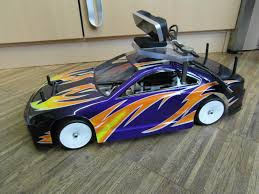
\includegraphics[width=0.5\textwidth]{./Figuras/Mini}
	\caption{AutoNOMOS Model.}
	\label{fig:auto}
\end{figure}
\par Los estudios desarrollados con estos vehículos abarcan el control de los mismos a través de distintas técnicas; tomando como ejemplo el trabajo de Juan Manuel Ibarraza et al.  \cite{juanmanuelibarrazannathaGeneracionTrayectoriasPara}, donde se investigó la generación de trayectorias para esta clase de vehículos mediante el control de modos deslizantes. En \cite{StreetMarkDetection} se realiza la detección de marcas del camino con una cámara web en combinación con una microcomputadora Raspberry Pi 2 a bordo de un vehículo a control remoto a escala 1:10; el vehículo está acondicionado con la computadora y la webcam a boro. La cámara trabaja en el espacio de color HSV, utilizando la librería OpenCV sobre la microcomputadora para realizar el procesamiento de la imagen, el cual emplea un filtrado gaussiano para el suavizamiento de la imagen.
\par Es importante mencionar al gran conjunto de investigaciones en torno a la conducción autónoma en vehículos de tamaño real, de donde han venido gran parte de las aportaciones. El DARPA Grand Challenge es de especial importancia al haber aportado vehículos como el Stanley o el Spirit o Berlin, cuyas aportaciones en el campo son la principal influencia para desarrollos más recientes como el Tesla Autopilot o el Google Waymo. A propósito del Spirit of Berlin, se rescata en \cite{javierrojoSpiritBerlinAutonomous2017} el informe técnico en el que se detallan los procedimientos seguidos por el equipo para la realización de este vehículo autónomo, al que llamaron {\it Spirit of Berlin} (Figura \ref{fig:Spirit}).
\begin{figure}[htbp!]
	\centering
	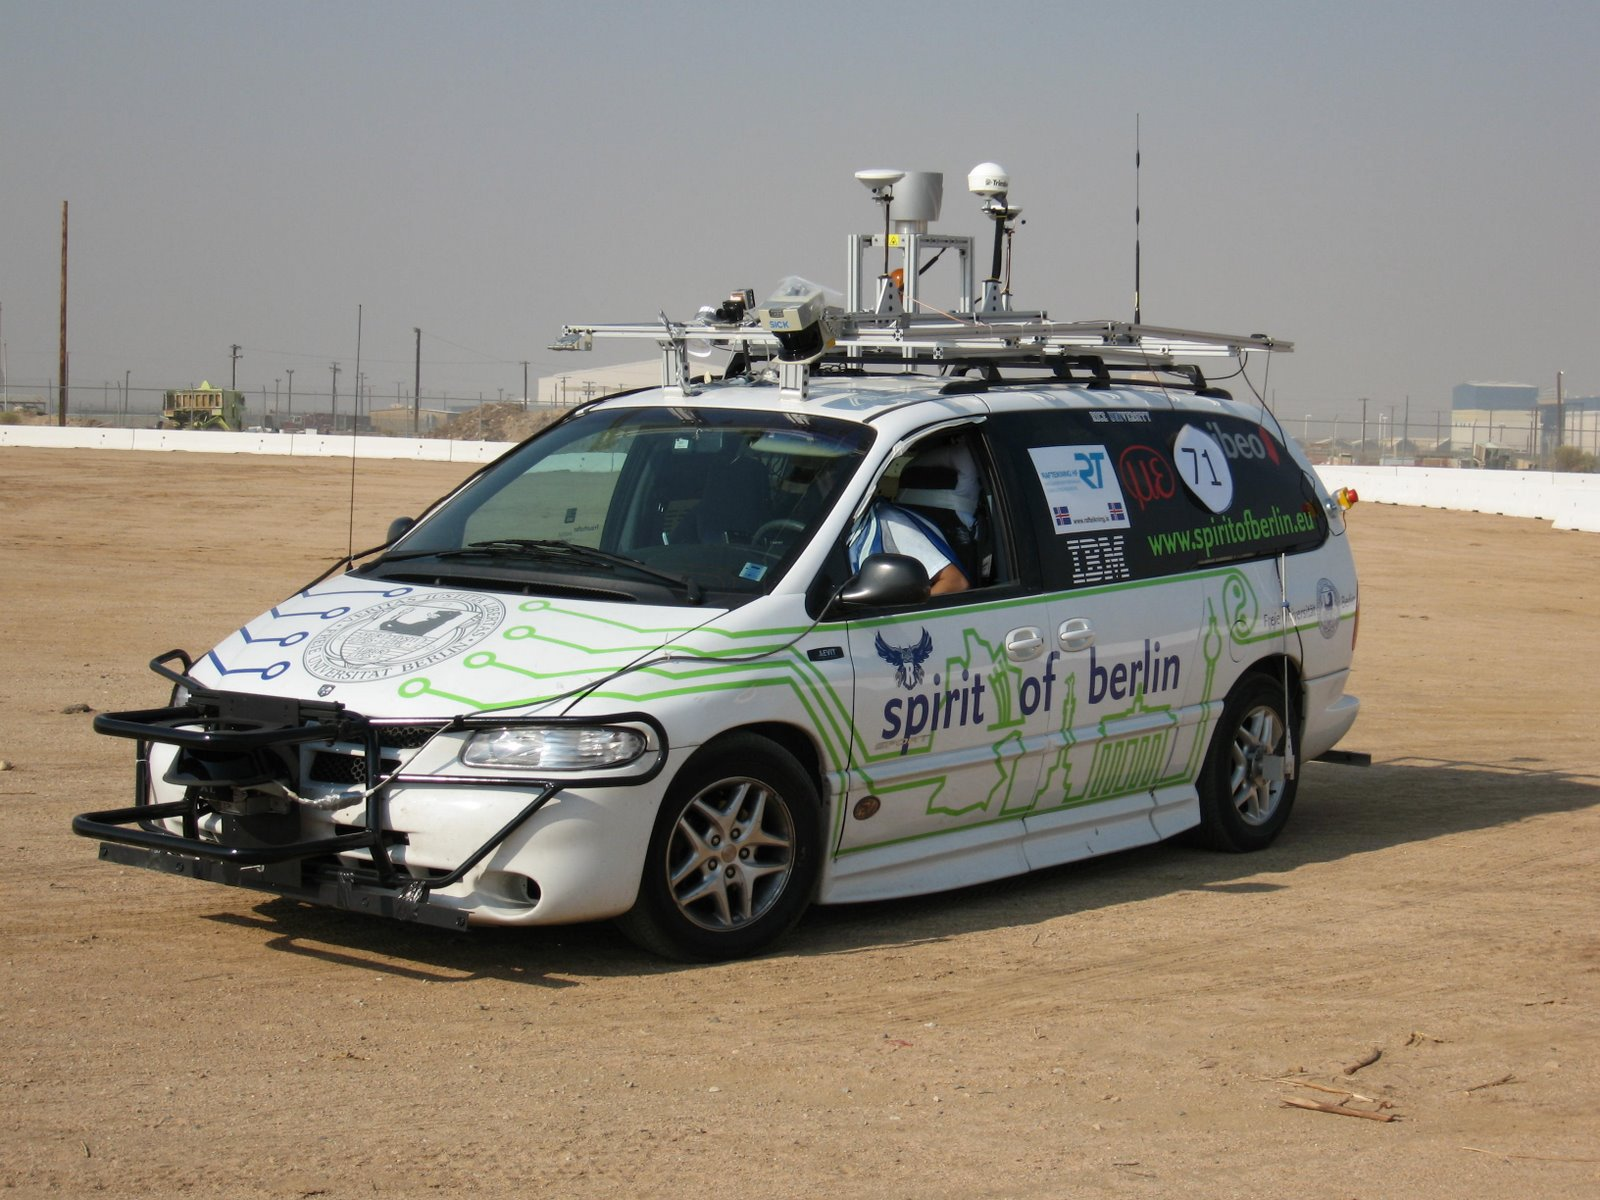
\includegraphics[width=0.5\textwidth]{./Figuras/SoB}
	\caption{Vehículo Spirit of Berlin, participante en el Darpa Grand Challenge.}
	\label{fig:Spirit}
\end{figure}
\par Las exploraciones alrededor vehículos autónomos, que se desencadenó con lo ya mencionado, ha llevado al desarrollo de nuevas técnicas de control enfocadas a esto; Katrakazas et al. mencionan en \cite{katrakazasRealtimeMotionPlanning2015} una perspectiva técnica histórica a través de varias investigaciones. Dentro del objetivo de buscar la autonomía, un grupo de investigadores chinos se encargó de desarrollar en \cite{wangLateralControlAutonomous2015} un controlador lateral para vehículos autónomos basado en lógica difusa. El sistema se basa en un controlador difuso tipo Mamdani y consiste en realizar el análisis del comportamiento de una trayectoria predefinida como referencia. La velocidad es considerada como un antecedente para las reglas de control difusas. Además de las simulaciones por computadora, los resultados se probaron con robots diferenciales del modelo IN$^{2}$BOT.
\par En \cite{marinoNestedPIDSteering2011}, Riccardo Marino et al. exploran las técnicas de preservación del carril para vehículos autónomos con base en un controlador PID no lineal con realimentación visual. En el modelo propuesto, la dinámica longitudinal se encuentra desacoplada de la dinámica lateral y puede ser despreciado para propósitos de control, lo cual permite linealizar el modelo. Esta investigación se simuló computacionalmente en el entorno CarSim, comparando los resultados con la respuesta de un conductor real. 
\par Sobre una investigación similar a la anterior, en \cite{leeSynthesisRobustLane2018} se aborda la preservación del carril, donde la planta es la dinámica lateral del vehículo, y el control tiene la característica de ser predictivo a pesar de las alteraciones exteriores que pudieran afectar la entrada. La investigación compara los resultados de simulación computacional entre un controlador PID, un regulador lineal cuadrático gaussiano, y un control tipo H$_{\infty}$. También en \cite{mackunisUnifiedTrackingRegulation2014}, se emplea una cámara monocular como sensor en un robot no-holónomo. El control se basa en el modelo geométrico de la perspectiva de la cámara a medida que el robot avanza, todo en el esquema IBVS.
\par Junto con la propia navegación autónoma surge la necesidad de contar con escenarios que faciliten este proceso a través de la propia comunicación de los vehículos con el entorno y viceversa; al respecto existen elementos importantes como AUTOPÍA, desarrollado en la Universidad Politécnica de Madrid en colaboración con la Universidad Complutense de Madrir, y esto es abordado por Pérez Rastelli en su tesis \cite{joshuemanuelperezrastelliAgentesControlVehiculos2012}, de donde se rescata la imagend e la Figura \ref{fig:Autopia}.
\begin{figure}[htbp!]
	\centering
	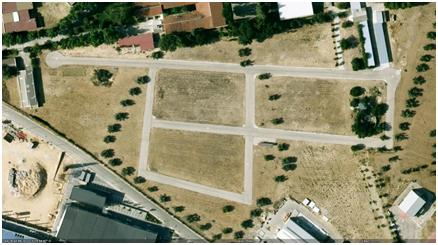
\includegraphics[width=0.5\textwidth]{./Figuras/AUTOPIA}
	\caption{Pista principal del proyecto AUTOPÍA.}
	\label{fig:Autopia}
\end{figure}